

\documentclass[runningheads,a4paper]{llncs}

\usepackage{amssymb}
\setcounter{tocdepth}{3}
\usepackage{graphicx}

\usepackage{url}
\urldef{\mailsa}\path|{alfred.hofmann, ursula.barth, ingrid.haas, frank.holzwarth,|
\urldef{\mailsb}\path|anna.kramer, leonie.kunz, christine.reiss, nicole.sator,|
\urldef{\mailsc}\path|erika.siebert-cole, peter.strasser, lncs}@springer.com|
\newcommand{\keywords}[1]{\par\addvspace\baselineskip
\noindent\keywordname\enspace\ignorespaces#1}

\usepackage{amsfonts}
\usepackage{bbm}
\usepackage{times}
\usepackage{latexsym,amsmath,amsfonts,mathrsfs}
\usepackage{amssymb}
\usepackage{amstext}
\usepackage{amsopn}
\usepackage{cite}
\usepackage[toc,page]{appendix}
\usepackage{tikz}











\usepackage{algorithm}
\usepackage{algorithmic}
\renewcommand{\algorithmiccomment}[1]{//#1}

\numberwithin{equation}{section}

\begin{document}

\mainmatter
\title{Packing-Based Approximation Algorithm for the -Set Cover Problem}

\titlerunning{Packing-Based Approximation Algorithm for the -Set Cover Problem}

\author{
Martin F\"{u}rer\thanks{Research supported in part by NSF Grant CCF-0728921 and CCF-0964655} \and Huiwen Yu
}
\institute{
Department of Computer Science and Engineering \\
The Pennsylvania State University, University Park, PA 16802, USA
}



\toctitle{Lecture Notes in Computer Science}
\tocauthor{Authors' Instructions}



\date{}
\maketitle



\begin{abstract}
We present a packing-based approximation algorithm for the -Set Cover problem. We introduce a new local search-based -set packing heuristic, and call it Restricted -Set Packing. We analyze its tight approximation ratio via a complicated combinatorial argument. Equipped with the Restricted -Set Packing algorithm, our -Set Cover algorithm is composed of the -Set Packing heuristic \cite{schrijver} for , Restricted -Set Packing for  and the semi-local -improvement \cite{furer} for 3-Set Cover. We show that our algorithm obtains a tight approximation ratio of , where  is the -th harmonic number. For small , our results are  for ,  for  and  for . Our algorithm improves the currently best approximation ratio for the -Set Cover problem of any .

\end{abstract}



\section{Introduction}

Given a set of elements  and a collection of subsets  of  with each subset of  having size at most  and the union of  being , the -Set Cover problem is to find a minimal size sub-collection of  whose union remains . Without loss of generality, we assume that  is closed under subsets. Then the objective of the -Set Cover problem can be viewed as finding a disjoint union of sets of  which covers .

The -Set Cover problem is NP-hard for any . For , the 2-Set Cover problem is polynomial-time solvable by a maximum matching algorithm. The greedy approach for approximating the -Set Cover problem chooses a maximal collection of -sets (sets with size ) for each  from  down to 1. It achieves a tight approximation ratio  (the k-th harmonic number) \cite{johnson}. The hardness result by Feige \cite{feige} shows that for , the Set Cover problem is not approximable within  for any  unless NPDTIME(). For the -Set Cover problem, Trevisan \cite{trevisan} shows that no polynomial-time algorithm has an approximation ratio better than  unless subexponential-time deterministic algorithms for NP-hard problems exist. Therefore, it is unlikely that a tremendous improvement of the approximation ratio is possible.

There is no evidence that the  lower bound can be achieved. Research on approximating the -Set Cover problem has been focused on improving the positive constant  in the approximation ratio . Small improvements on the constant might lead us closer to the optimal ratio. One of the main ideas based on greedy algorithms is to handle small sets separately. Goldschmidt et al. \cite{gold} give a heuristic using a matching computation to deal with sets of size 2 and obtain an  approximation ratio. Halld\'{o}rsson \cite{hall2} improves  to  via his ``t-change''  and ``augmenting path'' techniques. Duh and F\"{u}rer \cite{furer} give a semi-local search algorithm for the 3-Set Cover problem and further improve  to . They also present a tight example for their semi-local search algorithm.

A different idea is to replace the greedy approach by a set-packing approach. Levin \cite{levin} uses a set-packing algorithm for packing 4-sets and improves  to  for . Athanassopoulos et al. \cite{lp} substitute the greedy phases for  with packing phases and reach an approximation ratio  for .

The goal of this paper is not to provide incremental improvement in the approximation ratio for -Set Cover. We rather want to obtain the best such result achievable by current methods. It might be the best possible result, as we conjecture the lower bound presented in \cite{trevisan} not to be optimal.

In this paper, we give a complete packing-based approximation algorithm (in short, PRPSLI) for the -Set Cover problem. For , we use the -set packing heuristic introduced by Hurkens and Shrijver \cite{schrijver}, which achieves the best known to date approximation ratio  for the -Set Packing problem for any . On the other hand, the best hardness result by Hazan et al. \cite{hazan} shows that it is NP-hard to approximate the -Set Packing problem within .

For , we use the same packing heuristic with the restriction that any local improvement should not increase the number of 1-sets which are needed to finish the disjoint set cover. We call this new heuristic Restricted -Set Packing. We prove that for any , the Restricted -Set Packing algorithm achieves the same approximation ratio as the corresponding unrestricted set packing heuristic. For , this is not the case. The approximation ratio of the Restricted 4-Set Packing algorithm is , which is worse than the  ratio of the 4-set packing heuristic but it is also tight. For , we use the semi-local optimization technique \cite{furer}. We thereby obtain the currently best approximation ratio for the -Set Cover problem. Table 1 (in Appendix Section 5) includes a comparison of the approximation ratio of our algorithm with  \cite{furer}, Levin's algorithm \cite{levin} and  \cite{lp}. We also show that our result is indeed tight. Thus, -Set Cover algorithms which are based on packing heuristic can hardly be improved. Our novel Restricted -Set Packing algorithm is quite simple and natural, but its analysis is complicated. It
is essentially based on combinatorial arguments. We use the factor-revealing linear programming analysis for the -Set Cover problem. The factor-revealing linear program is introduced by Jain et al. \cite{lp1} for analyzing the facility location problem. Athanassopoulos et al. \cite{lp} are the first to apply it to the -Set Cover problem.

The paper is organized as follows. In Section 2, we give the description of our algorithm and present the main results. In Section 3, we prove the approximation ratio of the Restricted -Set Packing algorithm. In Section 4, we analyze our -Set Cover algorithm via the factor-revealing linear program.


\section{Algorithm Description and the Main Theorem}

In this section, we describe our packing-based -Set Cover approximation algorithm. We first give an overview of some existing results.

Duh and F\"{u}rer \cite{furer} introduce a semi-local -improvement for the 3-Set Cover problem. First, it greedily selects a maximal disjoint union of 3-sets. Then each local improvement replaces  3-sets with  3-sets, if and only if after computing a maximum matching of the remaining elements, either the total number of sets in the cover decreases, or it remains the same, while the number of 1-sets decreases. They also show that the -improvement algorithm gives the best performance ratio for the -Set Cover problem among all semi-local -improvement algorithms. The ratio is proved to be tight.

\begin{theorem}[\cite{furer}]
The semi-local -optimization algorithm for 3-Set Cover produces a solution with performance ratio . It uses a minimal number of 1-sets.
\end{theorem}

We use the semi-local -improvement as the basis of our -Set Cover algorithm. Other phases of the algorithm are based on the set packing heuristic \cite{schrijver}. For fixed , the heuristic starts with an arbitrary maximal packing, it replaces  sets in the packing with  sets if the resulting collection is still a packing. Hurkens and Shrijver \cite{schrijver} show the following result,

\begin{theorem}[\cite{schrijver}]
For all , the local search -Set Packing algorithm for parameter  has an approximation ratio .
\end{theorem}

The worst-case ratio is also known to be tight. We apply this packing heuristic for . For , we follow the intuition of the semi-local improvement and modify the local search of the packing heuristic, requiring that any improvement does not increase the number of 1-sets. We use the semi-local (2,1)-improvement for 3-Set Cover to compute the number of 1-sets required to finish the cover. Lemma 2.2 in \cite{furer} guarantees that the number of 1-sets returned by the semi-local (2,1)-improvement is no more than this number in any optimal solution. We compute this number first at the beginning of the restricted phase. Each time we want to make a replacement via the packing heuristic, we compute the number of 1-sets needed to finish the cover after making the replacement. If this number increases, the replacement is prohibited. To summarize, we call our algorithm the Restricted Packing-based -Set Cover algorithm (PRPSLI) and give the pseudo-code in Algorithm 1. For input parameter ,  is the parameter of the local improvement in Phase . For any , we set  in the same way as in Theorem 2. For , we set .

\begin{algorithm}
\caption{Packing-based -Set Cover Algorithm (PRPSLI)}
\begin{algorithmic}

\STATE \COMMENT{\textbf{\emph{ The -Set Packing Phase}}}
\FOR{ down to 7} \STATE Select a maximal collection of disjoint -sets.\REPEAT \STATE Select  -sets and replace them with  -sets. \UNTIL{there exist no more such improvements.} \ENDFOR

\STATE \COMMENT{\textbf{\emph{ The Restricted -Set Packing Phase}}}
\STATE Run the semi-local -improvement algorithm for 3-Set Cover on the remaining uncovered elements to obtain the number of 1-sets.
\FOR{ to 4}
\REPEAT \STATE Try to replace  -sets with  -sets. Commit to the replacement only if the number of 1-sets computed by the semi-local -improvement algorithm for 3-Set Cover on the remaining uncovered elements does not increase. \UNTIL{there exist no more such improvements.} \ENDFOR

\STATE \COMMENT{\textbf{\emph{ The Semi-Local Optimization Phase}}}
\STATE Run the semi-local -improvement algorithm on the remaining uncovered elements.

\end{algorithmic}
\end{algorithm}


The algorithm clearly runs in polynomial time. The approximation ratio of PRPSLI is presented in the following main theorem. For completeness, we also state the approximation ratio for the 3-Set Cover problem, which is obtained by Duh and F\"{u}rer \cite{furer} and remains the best result. Let  be the approximation ratio of the -Set Cover problem.

\begin{theorem}[Main]
For all , the Packing-based -Set Cover algorithm has an approximation ratio  for even  and ;  for odd  and ; ;
; .
\end{theorem}

\begin{remark}
For odd , the approximation ratio  is derived from the expression . We can further obtain the asymptotic representation of , i.e., . Similarly, for even , .
Finally,  and .
\end{remark}

\begin{remark}
Restriction on Phase 6 is only required for obtaining the approximation ratio  for even  and . In other cases, only restriction on Phase 5 and Phase 4 are necessary.
\end{remark}



We prove the main theorem in Section 4. Before that, we analyze the approximation ratio of the Restricted -Set Packing algorithm for  in Section 3. We state the result of the approximation ratio of the Restricted -Set Packing algorithm as follows.

\begin{theorem}[Restricted -Set Packing]
There exists a Restricted 4-Set Packing algorithm which has an approximation ratio . For all  and for any , there exists a Restricted -Set Packing algorithm which has an approximation ratio .
\end{theorem}

\begin{remark}
Without loss of generality, we assume that optimal solution of the Restricted -Set Packing problem also has the property that it does not increase the number of 1-sets needed to finish the cover of the remaining uncovered elements. This assumption is justified by Lemma 2 in Appendix 9.1.
\end{remark}

\section{The Restricted -Set Packing Algorithm}

We fix one optimal solution  of the Restricted -Set Packing algorithm. We refer to the sets in  as optimal sets. For fixed , a local improvement replaces  -sets with  -sets. We pick a packing of -sets  that cannot be improved by the Restricted -Set Packing algorithm. We say an optimal set is an \emph{-level set} if exactly  of its elements are covered by sets in . For the sake of analysis, we call a local improvement an \emph{--improvement} if it replaces  sets in  with  sets in . As a convention in the rest of the paper, small letters represent elements, capital letters represent subsets of , and calligraphic letters represent collections of sets. We first introduce the notion of blocking.

\subsection{Blocking}

The main difference between unrestricted -set packing and restricted -set packing is the restriction on the number of 1-sets which are needed to finish the covering via the semi-local (2,1)-improvement. This restriction can prohibit a local improvement. If any --improvement is prohibited because of an increase of 1-sets, we say there exists a . In Example 1 given in Appendix Section 6.1, we construct an instance of 4-set packing to help explain how blocking works.

We now define blocking formally. We are given a fixed optimal -set packing  of  and a -set packing  chosen by the Restricted -Set Packing algorithm. We consider all possible extensions of  to a disjoint cover of  by 1-sets, 2-sets and 3-sets. We order these extensions lexicographically, first by the number of 1-sets, second by the total number of 2-sets and 3-sets which are not within a -set of , and third by the number of 3-sets which are not within a -set of . We are interested in the lexicographically first extension. Notice that we pick this specific extension for analysis only. We cannot obtain this ordering without access to . We explain how we order the extensions in Example 2 (Appendix Section 6.2).

Suppose we finish the cover from the packing  with the lexicographically first extension. Let  be an undirected graph such that each vertex in  represents an optimal set. Two vertices are adjacent if and only if there is a 2-set in the extension intersecting with the corresponding optimal sets. Since the number of 2-sets and 3-sets not within an optimal set is minimized, there are no multiple edges in the graph. For brevity, when we talk about a node  in , we also refer to  as the corresponding optimal set. Moreover, when we say the \emph{degree} of a node , we refer to the number of neighbors of .


\begin{proposition}
 is a forest.
\end{proposition}

\begin{proposition}
For any , there is no 1-set inside an -level set. i.e. 1-set can only appear in -level sets.
\end{proposition}

\begin{proposition}
For any tree  in , there is at most one node which represents an -level set, such that the degree of the node is smaller than .
\end{proposition}

For any tree, if there exists a node with property in Proposition 3, we define it to be the root. Otherwise, we know that all degree 1 nodes represent -level sets. We define an arbitrary node not representing a -level set to be the root. If there are only -level sets in the tree, i.e. the tree degenerates to one edge or a single point, we define an arbitrary -level set to be the root. All leaves represent -level sets. (The root is not considered to by a leaf.) We call such a tree a \emph{blocking tree}. For any subtree, we say that the leaves \emph{block} the nodes in this subtree. We also call the set represented by a leaf a \emph{blocking set}.

We consider one further property of the root.

\begin{proposition}
Let .
In any blocking tree, there exists at most one node of either 0-level or 1-level that is of degree 2. If such a node exists, it is the root.
\end{proposition}

The proofs of Proposition 1 to 4 are given in Appendix Section 6.3.

Based on these simple structures of the blocking tree, we are now ready to prove the approximation ratio of the Restricted -Set Packing algorithm.

\subsection{Analysis of the Restricted 4-Set Packing Algorithm}

We prove in this section that the Restricted 4-Set Packing algorithm has an approximation ratio . We first explain how this  ratio is derived. We use the unit  defined in Example 1 (Appendix Section 6.1). Assume when the algorithm stops, we have  copies of  and a relatively small number of 3-level sets. We denote the -th copy of  by . For each  and , the set  in  and  are adjacent. This chain of 's starts from and ends at a 3-level set respectively. Then the performance ratio of this instance is slightly larger than . We first prove that the approximation ratio of the Restricted 4-Set Packing algorithm is at least .

Given , a collection of blocking trees. We assign 4 tokens to every element covered by sets chosen by the restricted packing algorithm. We say a set has a free token if after distributing the token, this set retains at least 7 tokens. We show that we can always distribute the tokens among all the optimal sets , so that there are at least 7 tokens in each optimal set.


\begin{proof}
We present the first round of redistribution. \\



\textbf{Round 1 - Redistribution in each blocking tree }. Every leaf in  has 4 free tokens to distribute. Every internal node  of degree  requests  tokens from a leaf. We consider each node with nonzero request in the reverse order given by breadth first search (BFS).


        \begin{itemize}
            \item If ,  requests 4 tokens from any leaf in the subtree rooted at  which has 12 tokens.
            \item If ,  has three children .  sends requests of 4 tokens to any leaf in the subtree rooted at , one for each subtree.  takes any two donations of 4 tokens.
            \item The root of degree  receives the rest of the tokens contributed by the leaves.
        \end{itemize}

\begin{proposition}
After Round 1, every internal node in  has at least 8 tokens, the root of degree  has  tokens.
\label{prop1-k4}
\end{proposition}

Proposition 5 is proved in Appendix Section 7.1. According to Proposition 4, we know that after the first round of redistribution every node has at least 8 tokens except any 0-level roots which are of degree 1 and any singletons in  which are 1-level sets. \\

We first consider the collection of 1-level sets  which are singletons in . Let  be such a 1-level set that intersects with a 4-set  chosen by the algorithm. Assume  also intersects with  other optimal sets .

We point out that no  belongs to . Otherwise suppose . Then there is a 1-2-improvement (replace  with  and ).

We give the second round of redistribution, such that after this round, every set in  has at least 7 tokens.
For optimal sets , consider each token request sent to  from . We say it is an \emph{internal request}, if , and  and  intersect with a set  chosen by the algorithm. Otherwise, we say it is an \emph{external request}. \\

\textbf{Round 2 - Redistribution for }.  sends  requests of one token to  if . For each node  in , internal requests are considered prior to external requests.

        For each request sent to  from ,
        \begin{itemize}
            \item If  has at least 8 tokens, give one to .
            \item If  has only 7 tokens. \\
            (1) If  is a leaf, it requests from the node which has received 4 tokens from it during the first round of redistribution.\\
            (2) If  is not a leaf,

            (2.1) If ,  requests a token from a leaf which has at least 8 tokens in the subtree rooted at .  

            (2.2) If  is a node in . Suppose  has children  and  belongs to the subtree rooted at .  requests from a leaf  which has at least 8 tokens in the subtree rooted at .
        \end{itemize}


We now prove the correctness of the second round of redistribution.

\begin{proposition}
Every singleton node  of level  has at most  requests. Every leaf has at most  internal requests. Every internal node of level  has at most  requests. The root of level  has at most  requests.
\end{proposition}


\begin{proposition}
Singleton node  can satisfy all the requests.
\end{proposition}


\begin{proposition}
The root  of level  and degree  can satisfy all the requests if .
\end{proposition}


\begin{proposition}
There is no external request sent to a root which is of level 0 and degree 1.
\end{proposition}


\begin{proposition}
Any external request sent from a leaf  can be satisfied.
\end{proposition}


\begin{proposition}
Any external request sent from an internal node of degree  can be satisfied.
\end{proposition}

\begin{proposition}
Any external request sent from an internal node  of degree 2 can be satisfied.
\end{proposition}

The proofs of Proposition 6 to 12 are given in Appendix Section 7.1. From Proposition 7, 8, 10, 11 and 12, we know that all requests can be satisfied. Hence after the second round of distribution, every set in  has at least 7 tokens. And from Proposition 9, we know that every root of level 0 and degree 1 retains 4 tokens. \\


We consider a root  which is a 0-level set of degree 1.  receives 4 tokens from leaf . Assume  is covered by  and  intersect with . We first prove that,

\begin{proposition}
,  does not receive any token request during Round 2 of redistribution.
\end{proposition}

The proof of Proposition 13 is given in Appendix Section 7.1. Based on Proposition 13, for any set , we can think of a token request from  to  as an internal request to . We describe the third round of redistribution.

\textbf{Round 3 - Redistribution for root of level 0 and degree 1}. Request 1 token from each of  following Round 2.

\begin{proposition}
.
\end{proposition}

The correctness of Round 3 follows from Proposition 14. The proof of Proposition 14 is given in Appendix Section 7.1. We thus prove that a root of level 0 and degree 1 has 7 tokens after the third round of redistribution.



Therefore, after the three rounds of token redistribution, each optimal set has at least 7 tokens, then the approximation ratio of the Restricted 4-Set Packing algorithm is at least . \qed
\end{proof}

We give the construction of tight example in Appendix Section 7.2. We thus conclude that the approximation ratio of the Restricted 4-Set Packing algorithm is .


\subsection{Analysis of the Restricted -Set Packing Algorithm, }

For , we prove that the approximation ratio of the Restricted -Set Packing algorithm is the same as the set packing heuristic \cite{schrijver}. For fixed , a local improvement can replace at most  sets with  sets. We prove that for any , there exists an , such that the approximation ratio of the Restricted -Set Packing algorithm is at least .

The proof strategy is similar to that of the Restricted 4-Set Packing algorithm. We first create a forest of blocking trees . We give every element covered by sets chosen by the algorithm one unit of tokens. We then redistribute the tokens among all the optimal sets. We claim that for , after redistribution, every optimal set gets at least  units of tokens. We use a different parameter of local improvement from Theorem 2. The algorithm still runs in polynomial time.

\begin{proof}
The first round of redistribution goes as follows. \\

\textbf{Round 1 - Redistribution in each blocking tree }. Every leaf in  has  units of free tokens to distribute. Every internal node  of degree  receives  units of tokens from a leaf. The root receives the remaining tokens.

\begin{proposition}
After Round 1, every node has at least 2 units of tokens, except singletons which are 1-level sets.
\end{proposition}

We consider the collection of 1-level sets  which are singletons in . Let  be such a 1-level set that intersects with a -set  chosen by the algorithm. Assume  intersects with  other optimal sets . \\

\textbf{Round 2 - Redistribution for }.
    \begin{itemize}
    \item For every singleton node of level  ():

    Send 1 unit of tokens each to arbitrarily  internal requests.
    \item If  receives one unit of tokens, we are done. Otherwise, pick an arbitrary singleton node  from . Let . Let  be a set intersecting with  while it does not intersect with any set in . (The existence of  follows from Proposition 6.)
    \item If  intersects with some singleton node which has at least 3 units of tokens, we move 1 unit to . Otherwise pick an arbitrary singleton node  which intersects with . Let  be a set intersecting with  while it does not intersect with any set in .
    \item Repeat this procedure and form a chain of singleton sets  such that  and  intersect with ,  and  intersect with a set  chosen by the algorithm, for , until


        (1) The chain ends when excluding , every set intersecting with  is not a singleton node. Denote the collection of such  by .

        Move 1 unit of tokens from any node in the collection of non-degenerate blocking trees which has at least 3 units of tokens to .

        (2) The chain ends where there exists a 1-level set  which intersects with , such that  starts another chain of length  which ends at  (as illustrated in Fig. 4 (Appendix Section 8.1)).


        Construct a graph , such that every vertex in the graph represents a node in a chain,  are connected, if the corresponding nodes intersect with a set  chosen by the algorithm. Consider every connected component  in . Equally distribute all tokens to every vertex in .







    \end{itemize}


The correctness of step (1) and step (2) follows from Proposition 16 and 17. We give the proofs in Appendix Section 8.2.
\begin{proposition}
The collection of non-degenerate blocking trees has at least  free units of tokens. After step (1), every set in  has 2 units of tokens.
\end{proposition}

\begin{proposition}
After step (2), every optimal set has at least  units of tokens.
\end{proposition}

We conclude that after the second round of redistribution, every optimal set gets at least  units of tokens. Therefore, the approximation ratio of the Restricted -Set Packing algorithm is at least . \qed
\end{proof}

Moreover, the tight example of the -set packing heuristic \cite{schrijver} can also serve as a tight example of the Restricted -Set Packing algorithm for . Hence, the approximation ratio of the Restricted -Set Packing algorithm is . \\




\section{Analysis of the Algorithm PRPSLI}

We use the factor-revealing linear program introduced by Jain et al. \cite{lp1} to analyze the approximation ratio of the algorithm PRPSLI. Athanassopoulos et al. \cite{lp} first apply this method to the -Set Cover problem. Notice that the cover produced by the restricted set packing algorithms is a cover which minimizes the number of 1-sets. In Appendix Section 9.1, we first show that for any , there exists a -set cover which simultaneously minimizes the size of the cover and the number of 1-sets in the cover. We then present the set-ups and notations of the factor-revealing linear program (LP).

The proof of Theorem 3 is similar as the proof of Theorem 6 in \cite{lp}. Namely, we find a feasible solution to the dual program of (LP), which makes the objective function of the dual program equal to the value of  defined in Theorem 3, thus  is an upper bound of the approximation ratio of PRPSLI. We give the proof of an upper bound of the approximation ratio of PRPSLI in Appendix Section 9.2. On the other side, we give an instance for each , such that PRPSLI does not achieve a better ratio than  on this instance in Appendix Section 9.3. We thus prove Theorem 3.\\



\bibliographystyle{plain}

\bibliography{ISAACbib}

\newpage



\section*{Appendix}

\section{Comparison on the Approximation Ratio of the -Set Cover Problem with Previous Works}

\begin{table}
\caption{Comparison on the Approximation Ratio of the -Set Cover Problem}
\begin{center}
\begin{tabular}{|c|c|c|c|c|}

  \hline
 & \cite{furer} & \cite{levin} & \cite{lp} & PRPSLI \\
  \hline
  3 & 1.3333 & 1.3333 & 1.3333 & 1.3333 \\
  4 & 1.5833 & 1.5808 & 1.5833 & 1.5208 \\
  5 & 1.7833 & 1.7801 & 1.7833 & 1.7333 \\
  6 & 1.9500 & 1.9474 & 1.9208 & 1.8667 \\
  7 & 2.0929 & 2.0903 & 2.0690 & 2.0190 \\
  8 & 2.2179 & 2.2153 & 2.1762 & 2.1262 \\
  9 & 2.3290 & 2.3264 & 2.2917 & 2.2413 \\
  10 & 2.4290 & 2.4264 & 2.3802 & 2.3302 \\
  20 & 3.0977 & 3.0952 & 3.0305 & 2.9779\\
  21 & 3.1454 & 3.1428 & 3.0784 & 3.0284\\
  50 & 3.9992 & 3.9966 & 3.9187 & 3.8683\\
  75 & 4.4014 & 4.3988 & 4.3178 & 4.2678\\
  100 & 4.6874 & 4.6848 & 4.6021 & 4.5520 \\
  \hline
  large  &  &  &  &  \\
  \hline
\end{tabular}
\end{center}
\end{table}


\section{Section 3.1}

\subsection{Example 1}

\begin{example}[Blocking]
Consider an instance  of the 4-Set Cover problem. Suppose there is an optimal solution  of the Restricted 4-Set Packing algorithm which consists of only disjoint 4-sets that cover all elements. Let , . Let  be a collection of 4-sets chosen by the algorithm.  is a collection of 1-level or 2-level sets. Denote the -th element of  by , for . If , we say that  covers the elements  and . Denote the following unit by ,



We visualize this construction in Fig. 1. Let each cube represent a 4-set in  and we place  vertically within a  square (not shown in the figure), such that each  intersects with one or two sets in .  are placed horizontally. Notice that  which intersects with  respectively are 1-level sets. The other 12 sets in  are 2-level sets.

 is a collection of 3-level sets. Notice that for our fixed optimal solution, all elements can be covered by 4-sets, so there is no 1-set needed to finish the cover. For given , when we compute an extension of the packing to a full cover via the semi-local (2,1)-improvement, assume the unpacked element of  () can only be covered by a 2-set intersecting with both  and , or it introduces a 1-set in the cover. The remaining unpacked elements of  and  can be covered arbitrarily by 2-sets and 3-sets. In unrestricted packing, one of the local improvements consists of replacing  by . However, in restricted packing, for , adding any  to the packing would create a 1-set covering the unpacked element of  during the semi-local (2,1)-improvement. Hence this local improvement is prohibited as a result of restricting on the number of 1-sets.

We remark that blocking can be much more complicated than in this simple example. As we shall see later in Section 3.2, for the Restricted 4-Set Packing problem, a 3-level set can initiate a blocking of many optimal sets.



\begin{figure}
\begin{center}

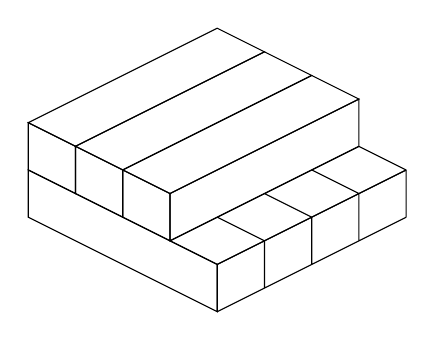
\begin{tikzpicture}[scale =0.6]

  \draw[yslant=-0.5] (0,0) rectangle (4,1);
  \draw[yslant=-0.5] (0,1) rectangle (1,2);
  \node at (0.5, 1.3) {};
  \draw[yslant=-0.5] (1,1) rectangle (2,2);
  \node at (1.5, 0.8) {};
  \draw[yslant=-0.5] (2,1) rectangle (3,2);
  \node at (2.5, 0.3) {};



  \draw[yslant=0.5] (4,-4) grid (8,-3);
  \node at (4.5,-1.3) {};
  \node at (5.5, -0.8) {};
  \node at (6.5, -0.3) {};
  \node at (7.5, 0.2) {};
\pgftransformyshift{1.5cm}
  \pgftransformxshift{-1cm}
  \draw[yslant=0.5] (4,-4) rectangle (8,-3);
  \pgftransformyshift{-1.5cm}
  \pgftransformxshift{1cm}

\pgftransformyshift{-2cm}
  \draw[yslant=0.5,xslant=-1] (4,4) rectangle (8,3);
  \draw[yslant=0.5,xslant=-1] (4,3) rectangle (8,2);
  \draw[yslant=0.5,xslant=-1] (4,2) rectangle (8,1);
  \pgftransformyshift{-1cm}
  \draw[yslant=0.5,xslant=-1] (4,1) grid (8,0);

\end{tikzpicture}
\caption{Placement of  to }
\end{center}
\end{figure}

\end{example}


\subsection{Example 2}
\begin{example}[Finish the cover by 1-sets, 2-sets and 3-sets]
In Fig. 2, Fig. 3 and Fig. 4. Rectangles placed vertically represent optimal sets. Circles represent 1-sets. Ellipses placed horizontally represent 2-sets or 3-sets, where the smaller ones stand for 2-sets and the larger ones stand for 3-sets. The cross symbol represents an element covered by a -set in . Let  be an ordered pair, such that,  is the number of 1-sets,  is the total number of 2-sets and 3-sets which are not within one optimal set, and  is the number of 3-sets which are not within one optimal set. These 1-sets, 2-sets and 3-sets are used to finish the cover. The right picture is always a cover which is before the cover in the left picture in the lexicographic order.
\end{example}

\begin{figure}
\begin{center}

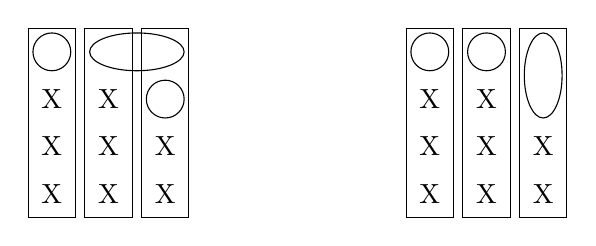
\begin{tikzpicture}[scale =0.6]
    \draw (0,0) rectangle (1,4);
    \draw (1.2,0) rectangle (2.2,4);
    \draw (2.4,0) rectangle (3.4,4);

    \draw (0.5,0.5) node {X} (0.5,1.5) node {X} (0.5,2.5) node {X} (1.7,0.5) node {X} (1.7,1.5) node {X} (1.7,2.5) node {X} (2.9,0.5) node {X} (2.9,1.5) node {X};

    \draw (0.5, 3.5) circle (0.4);
    \draw (2.3,3.5) ellipse (1 and 0.4);
    \draw (2.9, 2.5) circle (0.4);

    \node at (5.8, 2) {};
\pgftransformxshift{8cm}
    \draw (0,0) rectangle (1,4);
    \draw (1.2,0) rectangle (2.2,4);
    \draw (2.4,0) rectangle (3.4,4);

    \draw (0.5,0.5) node {X} (0.5,1.5) node {X} (0.5,2.5) node {X} (1.7,0.5) node {X} (1.7,1.5) node {X} (1.7,2.5) node {X} (2.9,0.5) node {X} (2.9,1.5) node {X};

    \draw (0.5, 3.5) circle (0.4);
    \draw (2.9,3) ellipse (0.4 and 0.9);
    \draw (1.7, 3.5) circle (0.4);

\end{tikzpicture}

\caption{}
\end{center}
\end{figure}


\begin{figure}
\begin{center}

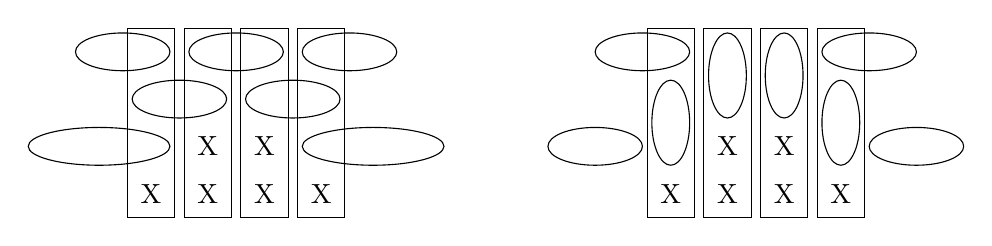
\begin{tikzpicture}[scale =0.6]
    \draw (0,0) rectangle (1,4);
    \draw (1.2,0) rectangle (2.2,4);
    \draw (2.4,0) rectangle (3.4,4);
    \draw (3.6,0) rectangle (4.6,4);
    \draw (0.5,0.5) node {X} (1.7,0.5) node {X} (1.7,1.5) node {X} (2.9,0.5) node {X} (2.9,1.5) node {X} (4.1,0.5) node {X};
    \draw (-0.1,3.5) ellipse (1 and 0.4);
    \draw (1.1, 2.5) ellipse (1 and 0.4);
    \draw (-0.6, 1.5) ellipse (1.5 and 0.4);
    \draw (2.3,3.5) ellipse (1 and 0.4);
    \draw (3.5, 2.5) ellipse (1 and 0.4);
    \draw (4.7, 3.5) ellipse (1 and 0.4);
    \draw (5.2, 1.5) ellipse (1.5 and 0.4);

    \node at (8, 2) {};
\pgftransformxshift{11cm}
    \draw (0,0) rectangle (1,4);
    \draw (1.2,0) rectangle (2.2,4);
    \draw (2.4,0) rectangle (3.4,4);
    \draw (3.6,0) rectangle (4.6,4);
    \draw (0.5,0.5) node {X} (1.7,0.5) node {X} (1.7,1.5) node {X} (2.9,0.5) node {X} (2.9,1.5) node {X} (4.1,0.5) node {X};
    \draw (-0.1,3.5) ellipse (1 and 0.4);
    \draw (0.5, 2) ellipse (0.4 and 0.9);
    \draw (-1.1, 1.5) ellipse (1 and 0.4);
    \draw (1.7,3) ellipse (0.4 and 0.9);
    \draw (2.9,3) ellipse (0.4 and 0.9);
    \draw (4.7, 3.5) ellipse (1 and 0.4);
    \draw (4.1,2) ellipse (0.4 and 0.9);
    \draw (5.7, 1.5) ellipse (1 and 0.4);
\end{tikzpicture}


\caption{}
\end{center}
\end{figure}


\begin{figure}
\begin{center}
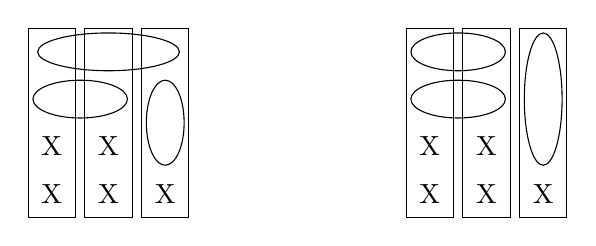
\begin{tikzpicture}[scale=0.6]

    \draw (1.2,0) rectangle (2.2,4);
    \draw (2.4,0) rectangle (3.4,4);
    \draw (3.6,0) rectangle (4.6,4);
    \draw (1.7,0.5) node {X} (1.7,1.5) node {X} (2.9,0.5) node {X} (2.9,1.5) node {X} (4.1,0.5) node {X};
    \draw (2.9,3.5) ellipse (1.5 and 0.4);
    \draw (2.3, 2.5) ellipse (1 and 0.4);
    \draw (4.1, 2) ellipse (0.4 and 0.9);

    \node at (7, 2) {};
    \pgftransformxshift{8cm}
    \draw (1.2,0) rectangle (2.2,4);
    \draw (2.4,0) rectangle (3.4,4);
    \draw (3.6,0) rectangle (4.6,4);
    \draw (1.7,0.5) node {X} (1.7,1.5) node {X} (2.9,0.5) node {X} (2.9,1.5) node {X} (4.1,0.5) node {X};
    \draw (2.3,3.5) ellipse (1 and 0.4);
    \draw (2.3, 2.5) ellipse (1 and 0.4);
    \draw (4.1, 2.5) ellipse (0.4 and 1.4);

\end{tikzpicture}
\caption{}
\end{center}
\end{figure}

\subsection{Proofs in Section 3.1}

\begin{proof}[Proposition 1]
It is sufficient to show that there is no cycle in . Suppose  form a cycle in . We remove the 2-sets intersecting with adjacent nodes in the cycle and add the 2-sets inside each , for . Then the total number of 2-sets and 3-sets not within an optimal set decreases. \qed
\end{proof}

\begin{proof}[Proposition 2]
Let  be an -level set which is covered by a 1-set, for . If there are more than one 1-set covering , we can replace them with 2-set or 3-set inside . Hence we only consider the case that there is only one 1-set covering . If there is a 2-set or 3-set inside , we can remove the 1-set and replace the 2-set or 3-set with a 3-set or two 2-sets respectively. If  is a singleton node, since , there exists a 2-set or 3-set inside . Otherwise let  be any node of degree 1 which connects to  via a simple path . We remove all 2-sets intersecting with adjacent nodes in this path and move the 1-set from  to , then add 2-sets inside . If there is a 1-set in any , , it can be replaced together with the 2-set just added inside  with a 3-set. If there is another 1-set in , it can be combined with the 1-set moved from  to a 2-set. Hence, there is no 1-set in any -level set for . \\ However, 1-set can remain in -level set. In this case, the -level set is a singleton node in . \qed
\end{proof}

\begin{proof}[Proposition 3]
We consider non-degenerate tree. Suppose there are two nodes, an -level set  and a -level set  which satisfy the requirements. Consider a simple path connecting  and . We remove all 2-sets intersecting with adjacent nodes on this simple path. For those nodes excluding  on the path, we can add a 2-set inside each optimal set. For , since  is not a -level set, there is no 1-set inside . Moreover, the degree of  is smaller than , hence there is a 2-set or 3-set inside , we can then replace it with a 3-set or two 2-sets inside  respectively. The same argument applies to . Hence, there can be at most one -level set with degree smaller than . \qed
\end{proof}

\begin{proof}[Proposition 4]
We first prove that there is at most one node of either 0-level or 1-level which is of degree 2. Assume  and  are 0-level or 1-level sets and of degree 2. We replace the 2-sets intersecting with two adjacent nodes along the simple path connecting  and  with 2-sets or 3-sets inside the optimal sets represented by these nodes, then the total number of 2-sets and 3-sets not within an optimal set decreases. In this way,  and  turn to be of degree 1.

Suppose we have one 0-level or 1-level set  of degree 2. We prove that there is no node of degree 1 representing an -level set for any , thus  is the root. Assume  is an -level set of degree 1. We replace the 2-sets intersecting with two adjacent nodes along the simple path connecting  and  with 2-sets or 3-sets inside the optimal sets represented by these nodes, then the total number of 2-sets and 3-sets not within an optimal set decreases. In this way,  turns to be of degree 1 and  turns to be of degree 0. \qed
\end{proof}


\section{Section 3.2}

\subsection{Proofs in Section 3.2}

\begin{proof}[Proposition 5]
Consider any subtree with root  of degree ,  ( is not the root of ). Since any internal node of degree 2 does not request any token, for simplicity we assume there is no internal node of degree 2 in the subtree. Assume  has children . If every child of  is a leaf, since the request is processed in the reverse order given by BFS, we know that there is no other node requesting tokens from , hence 's requests can be satisfied. Assume that in every subtree rooted at , all the requests have been satisfied. Since for any tree with root of degree , the quantity

equals to the number of the leaves of the tree. We know that there are 4 free tokens in each subtree rooted at . Hence, 's requests can be satisfied.

By (\ref{eqn:node}), the root of  receives  tokens. \qed
\end{proof}

\begin{proof}[Proposition 6]
Suppose a singleton node  is covered by . If every  intersects with , we have a local improvement by replacing  with  and . Hence,  intersect with at most  sets in .  has at most  requests of tokens. Similarly, we know that a leaf is a -level set, it has at most  internal requests.

Every internal node of level  can have  requests, and the root of level  can have  requests. \qed
\end{proof}


\begin{proof}[Proposition 7]
Assume  is of level  and . From Proposition 6,  has at most  request. After giving  tokens,  has  tokens left. Hence,  can satisfy all the requests. \qed
\end{proof}

\begin{proof}[Proposition 8]
The root has  tokens and it has at most  requests. If it has at most  requests, it retains  tokens after satisfying all the requests.

It remains to prove that it cannot have  requests. Otherwise, suppose  is covered by  and every  intersects with . There are leaves  which request token from  for 1-level singleton .  intersects with . Then we have a --improvement (replace  with  and ). \qed
\end{proof}

\begin{proof}[Proposition 9]
If such a root has an external request from , then  is a leaf and  has an internal request from an ,  intersects with an . Then we have a 1-2-improvement (replace  with  and the root). \qed
\end{proof}


\begin{proof}[Proposition 10]
By Proposition 6,  makes an external request if and only if it has 2 internal requests. As in Step (1),  sends request to  which has received 4 tokens from it. If  has at least 8 tokens, it gives one to . Otherwise, we proceed with Step (2.2). Hence, it is sufficient to prove that in (2.2), there exists a leaf in some subtree rooted at  which has 8 tokens.

Otherwise, suppose any leaf in the subtree rooted at  has an internal request. We pick  belonging to the subtree rooted at  respectively.  has an internal request from  which intersects with . Moreover, we know that  has an internal request from  intersecting with . We have a --improvement (replace  with  and ). \qed
\end{proof}

\begin{proof}[Proposition 11]
An internal node of degree at least 3 sends a request if and only if it receives a request from a leaf but fails to satisfy it. The proof is indeed contained in the proof of Proposition 10. \qed
\end{proof}


\begin{proof}[Proposition 12]
If  makes an external request, by Proposition 6,  has two internal requests, say from .  intersects with ,  intersects with .

Let  be a closest node to  which belongs to the subtree rooted at  and has a degree . If no such  exists, let  and . If on the contrary, 's request cannot be satisfied, we pick a leaf in each subtree rooted at a child of . Let  be these leaves, then  has an internal request from  intersecting with . We then have a local improvement by replacing  with ,  and . \qed
\end{proof}


\begin{proof}[Proposition 13]
First, . Otherwise, assume  intersects with , we have a 1-2-improvement (replace  with  and ). Hence,  does not have any internal request.

 does not have any external request either. Recall in Round 2 of redistribution, a leaf has an external request if there exists an internal node  of degree , such that  belongs to the subtree rooted at , and \\
- If ,  has two internal requests from ,  intersect with  respectively. However in this case, we have a 3-4-improvement (replace  with ).\\
- If , there is an external request sent to  from leaf ,  has an internal request from  which intersects with , and there is an internal request sent to  from . Let  intersect with . We have a 3-4-improvement (replace  with ). \\
- If , there are two external requests sent to  from leaves .  have internal requests from .  intersect with  respectively. There is a 3-4-improvement (replace  with ).

Hence,  does not have any token request during Round 2 of redistribution. \qed
\end{proof}


\begin{proof}[Proposition 14]
First, . Otherwise, we have a 1-2-improvement (replace  with  and ).  \\
If , then the number of elements contained in
 is . Hence . If , there exists an  which is a 3-level set and completely covered by . However in this case, we have a 2-3-improvement (replace  with ). Hence, . \\
If , then the number of elements contained in
 is . In this case, .  \qed
\end{proof}

\subsection{Tight example of the Restricted 4-Set Packing algorithm}

We construct an example showing that for any fixed , which is the parameter of the local improvement, and any  and there exists an instance, on which the Restricted 4-Set Packing algorithm has a performance ratio at most . We thereby conclude that the approximation ratio of the Restricted 4-Set Packing algorithm is . \\

Our construction is randomized. We take  copies of the unit  defined in Example 1. Then there are  2-level sets. Suppose there are  3-level sets which start the blocking. In case of 4-set packing, blocking can start from a single 3-level set , then propagate through an arbitrary number of 2-level sets  (). More specifically, we form the blocking by covering the remaining uncovered elements of  by 2-sets , such that  intersects  and , for .

In our example, we assign each 2-level set to one of the  blocking sets independently and uniformly at random. If a 2-level set is assigned to a blocking set, that blocking set is a leaf of the blocking tree containing the 2-level set. For fixed , we consider local --improvements for any . For each subset of  with size , suppose after removing one covering set of  blocking sets, we can replace these  sets with at most  optimal sets. Then . If , i.e., , there is a local improvement. \\

We assume . Let  be the maximum number of 2-level sets which can be added to the solution by the local improvement. Then . Let  be the collection of 2-level sets. Let  be a set of random variables, where  is the number of nonempty subsets of  with size at most . Assume we enumerate every 2-level sets and arrange all subsets of  lexicographically. Let  be the event that there exists a local improvement which adds the -th subset with size at most  of  to the solution. Let  be the number of blocking sets assigned to the 2-level sets in this subset. Then,



Since the assignments of 2-level sets to blocking sets are independently and uniformly at random, we bound (7.2) as follows,



Assume that . Since each  depends on less than  elements in , and . By the following lemma, we have .

\begin{lemma}[Corollary 5.12 \cite{random}]
Let  be events in a probability space with  for all . If each event is mutually independent of all other events except for at most , and , then .
\end{lemma}

Therefore, there exists an assignment of 2-level sets to blocking sets such that no local --improvement is possible, for . \\

Assume all 3-level sets but a constant few of them are blocking sets. The performance ratio of the Restricted 4-Set Packing algorithm on this instance is . The ratio tends arbitrarily close to  when .



\section{Section 3.3}

\subsection{Figure 5}

\begin{figure}
\begin{center}
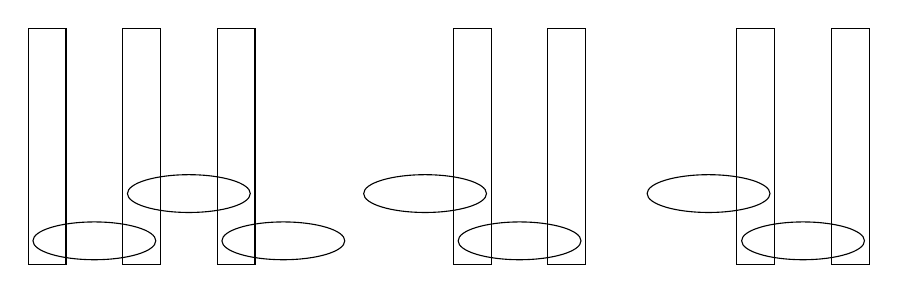
\begin{tikzpicture}[scale=0.6]

    \draw (0,0) rectangle (0.8,5); \node at (0.4, 4.5) {};
    \draw (2,0) rectangle (2.8,5); \node at (2.4,4.5) {};
    \draw (4,0) rectangle (4.8,5); \node at (4.4,4.5) {};
    \draw (1.4, 0.5) ellipse (1.3 and 0.4); \node at (1.4,0.5) {};
    \draw (3.4,1.5) ellipse (1.3 and 0.4); \node at (3.4, 1.5) {};
    \draw (5.4, 0.5) ellipse (1.3 and 0.4); \node at (5.4, 0.5) {};

    \node at (6.5, 2.5) {};

    \pgftransformxshift{2cm};
    \draw (7,0) rectangle (7.8,5); \node at (7,4.5) {};
    \draw (9,0) rectangle (9.8,5); \node at (9.4,4.5) {};

    \node at (11.5,2.5) {};
    \draw (13,0) rectangle (13.8,5); \node at (13.4, 4.5) {};
    \draw (15,0) rectangle (15.8,5); \node at (15.4,4.5) {};


    \draw (6.4, 1.5) ellipse (1.3 and 0.4); \node at (6.4,1.5) {};
    \node at (8.4,0.5) {};
    \draw (8.4,0.5) ellipse (1.3 and 0.4);
    \draw (12.4, 1.5) ellipse (1.3 and 0.4);
    \node at (12.4,1.5) {};
    \draw (14.4,0.5) ellipse (1.3 and 0.4); \node at (14.4, 0.5) {};


\end{tikzpicture}
\caption{Rectangles represent optimal -sets. Ellipses represent -sets chosen by the algorithm.}
\end{center}
\end{figure}

\subsection{Proofs in Section 3.3}

\begin{proof}[Proposition 15]
According to Proposition 4 and (\ref{eqn:node}), we know that after Round 1, every node has at least 2 units of tokens except singletons which are 1-level sets. Note that contrary to the Restricted 4-Set Packing problem, in restricted -set packing for , every leaf contributes at least 2 units of tokens. Hence, even if a root is of level 0 and degree 1, it can still receives at least 2 units of tokens after the first round of redistribution.

We remark that we do not care about from which leaf an internal node or the root receive the tokens. \qed
\end{proof}

\begin{proof}[Proposition 16]
Let . Without loss of generality, assume there is only one non-degenerate tree . Let  have an -level root of degree  and a set of internal nodes with degree set .

From (\ref{eqn:node}), we know that the leaves contribute  units of tokens. Here the summation goes through the set of internal nodes. There are , i.e.  free units of tokens in  which can be distributed to sets in . \\
Assume on the contrary that
        

        We derive an upper bound on .

        We first claim that any . If , we know that  has at least 3 units of tokens.

        If , the  elements of  which do not intersect with , intersect with . If , for each , there are  corresponding elements intersecting with . Here, these  elements belong to . Hence,  covers at least  elements. On the other hand, there are  elements covered by . We have,
        
        Combining (\ref{N1lb}) and (\ref{N1ub}), we get , which implies
        
        (\ref{dv1}) only holds for the case that  and there are at most 2 internal nodes. In this case, we observe that the leaf cannot intersect with any set  which intersects with , or we have a 1-2-improvement by replacing  with  and the root. Hence, we modify (\ref{N1ub}) and get
        
        Combining (\ref{N1ub2}) and (\ref{N1lb}), we have . Since , it leads to a contradiction. \qed
\end{proof}

\begin{proof}[Proposition 17]
Let  be the number of edges and  be the number of vertices in .

If  contains a circle, then . The average number of tokens in  is .

If  is a tree, then . We claim that . Otherwise, there exists a --improvement (replace all the sets corresponding to edges in  with all the sets corresponding to vertices in ). The average number of tokens in  is  for .

Hence, in any case, after collecting all tokens of  then equally distributed among every vertex in , each vertex gets at least  units of tokens.  \qed
\end{proof}


\section{Proof of Theorem 3}

\subsection{Set-up of the Factor-revealing LP}

We first prove that there exists a -set cover which simultaneous minimizes the size and the number of 1-sets in the cover.
\begin{lemma}
Suppose there are -set covers , , where  has  sets and  1-sets, and  has  sets and  1-sets. Then there exists a -set cover  which has  sets and  1-sets.
\end{lemma}

\begin{proof}
We create a bipartite graph , where every vertex in () represents a set in ( ), and every edge in  represents an element in the universe. Hence, the degree of a vertex represents the size of the corresponding set. Two vertices being adjacent means the corresponding two sets covers a same element. We show how to find .
 
For simplicity, assume  is connected and . If , take  to be . Otherwise, consider a vertex  of degree 1 such that its neighbor has degree at least 2. If there exists a vertex  of degree at least 3, assume  is the one with the shortest distance to . Consider the path  connecting  and , we replace the corresponding sets of  with  and delete the element in  which is covered by both  and . If any  () has degree at least 3, delete the elements in  which are not covered by . In this way,  decreases by 1 while  remains the same. If there is no  which has degree at least 3, since , and  and  cover the same universe of elements,  must be greater than , a contradiction. Hence, we can eventually decrease  to be at most . Finally, we take  to be this modified . \qed

\end{proof}

We are now ready to set-up the factor-revealing linear program for the -set cover problem.

Let  be an instance of the -Set Cover problem, where  is the set of elements to be covered,  is a collection of sets, and . For , let  be the instance for phase  of Algorithm PRPSLI, where  is the set of elements which have not been covered before Phase  and  is the collection of sets in  which contain only the elements in . Let  be an optimal solution of  for . For ,  is an optimal solution of  with minimal number of 1-sets.  is an optimal solution of . Let  be the ratio of the number of -sets in  over the number of sets in . Let  be the approximation ratio of the set packing algorithm used in Phase . Let  be the ratio of the number of -sets chosen by the semi-local optimization phase over the number of sets in . Since , we have for ,


In each phase of PRPSLI, the number of -sets chosen by the algorithm is . Since , then . Let  be the approximation ratio of the set packing algorithm used in Phase . At the beginning of Phase , there are  -sets. Thus,

i.e.


We consider additional constraints imposed by the restricted phases, namely for Phase 6 to 3. Let  be the ratio of the number of -sets chosen by the semi-local optimization phase over the number of sets in , for . In each restricted phase, the number of 1-sets does not increase. Hence, for ,


Next, we obtain an upper bound of the approximation ratio of PRPSLI. From Lemma 2.3 in \cite{furer}, we have . Also notice that . Thus we have an upper bound of , namely,


Combining (9.2) and (9.6), we have an upper bound of the approximation ratio of PRPSLI as,


Moreover,



Hence, we define the factor-revealing linear program of PRPSLI with objective function (9.7) and constraints (9.1), (9.4), (9.5), (9.8), (9.9) as follows,



We also prove that

\begin{lemma}
For any , the approximation ratio of Algorithm PRPSLI is upper-bounded by the maximized objective function value of the factor-revealing linear program (LP).
\end{lemma}


\subsection{Finding an Upper bound for the approximation ratio of PRPSLI}

\begin{proof}

Plug  for  and  in (LP). The dual of (LP) is,







For , set , , . We have . \\

For , set , , . We have . \\

For .\\

Set ; ,  for , , ; ,  for , . \\

For , . By induction, . Hence,


Then, constraints (2),(3) and (4) hold as equality. \\

In constraint (6) for , , . \\

In constraint (8) for , inequalities hold as equality. \\

Constraint (9) holds, . \\

Constraint (10) holds as equality. \\

Set , , ,  for odd  and  for even . \\

, . Let , . \\


For  is odd and ,  increases monotonically with respect to . Thus, for any odd  and ,  .\\
For , . \\

Hence, Constraint (1) holds, . \\

For  is even and ,  decreases monotonically with respect to .
For , . Thus, for any even  and , . Moreover, 

Hence, Constraint (1) holds, . \\

Constraint (5) for , constraint (6) for , constraint (7) and constraint (8) for  hold directly as a result of the settings of these parameters. \\

Constraint (5) for  holds, .\\

Constraint (9.1) holds for , . \\

Moreover, constraint (11), (12), (13) hold. \\

Finally, we compute the value of the objective function. \\

For odd  and ,
. \\

Last inequality holds because . \\

Similarly, for even  and , . \\


Therefore, the approximation ratio of PRPSLI for odd  and  can be upper bounded by . For even  and , it is upper bounded by . \qed
\end{proof}


\subsection{Tight example of PRPSLI}
For every  and any , we give a tight example of PRPSLI based on the tight example of the semi-local -improvement \cite{furer} for 3-Set Cover, the tight example of the Restricted 4-Set Packing algorithm we give in Appendix Section 7.2, and the tight example of the Restricted -Set Packing algorithm for , which is the same as the tight example of the -set packing heuristic \cite{schrijver}. \\

We assume that the optimal solution  consists of only disjoint -sets. To calculate the performance ratio on this instance, we charge a cost of 1 for each set chosen by the algorithm, and the cost is uniformly distributed to every element of the chosen set \cite{furer}.

\begin{itemize}

    \item \textbf{}. In Phase 4, the Restricted 4-Set Packing algorithm covers 1 element of each set in a  fraction of , 2 elements of each set in a  fraction, and 3 elements of each set in the remaining  fraction. Denote the three parts of  by ,  and  respectively. In Phase 3, the semi-local optimization covers 1 element in each set of  by 3-sets, and the remaining uncovered elements of  are covered by 2-sets. The performance ratio of PRPSLI on this instance is . \\

    \item \textbf{}. In Phase 5, the Restricted 5-Set Packing algorithm covers 2 elements of each set in a  fraction of , 1 element of each set in the remaining  fraction. Denote the two parts of  by  and  respectively. The algorithm switches to 4-Set Cover on  and it performs a semi-local optimization on . The performance ratio of Algorithm 1 on this instance is . \\

    \item \textbf{ odd and }. In Phase , the -Set Packing algorithm covers 2 elements of each set in a  fraction of , 1 element of each set in the remaining  fraction. Denote the two parts of  by  and  respectively. In Phase , the algorithm covers 1 element of each set in . Then it switches to -Set Cover on the remaining uncovered elements. The performance ratio of PRPSLI on this instance is at least , i.e. , which is  for , and by induction   for . The coefficient of  is upper bounded by . Hence, the performance ratio is at most  for . \\

    \item \textbf{ even and }. In Phase , the -Set Packing algorithm covers 2 elements of each set in a  fraction of , 1 elements of each set in the remaining  fraction. Denote the two parts of  by  and  respectively. In Phase , the -Set Packing algorithm covers 1 element of each set in  and then 1 element of each set in . Then the algorithm switches to -Set Cover on the remaining uncovered elements. The performance ratio of Algorithm 1 on this instance is at least , i.e. , which is  for  and by a similar argument as the above case, at most  for . \\

\end{itemize}



\end{document}
